\section{Blur}

\subsection{Introducción}
Blur es un filtro que suaviza la imagen. Esto lo hace asignándole a cada píxel el promedio (media aritmética) con sus píxeles vecinos. Es decir:

$$m_{i, j} = (m_{i-1, j-1} + m_{i-1, j} + m_{i-1, j+1} + m_{i, j-1} + m_{i, j} + m_{i, j+1} + m_{i+1, j-1} + m_{i+1, j} + m_{i+1, j+1}) / 9$$

Las consecuencias de adoptar este método son fundamentalmente dos; en primer lugar, nótese que esto significa que no vamos a procesar los píxeles en los bordes, ya que no tienen la cantidad suficiente de píxeles vecinos.

En segundo lugar, debemos tener en cuenta que el cálculo de blur en particular requiere utilizar datos de los elementos aledaños en la matriz, por lo que es imposible procesar la imagen con una complejidad espacial de $O(1)$, de cualquier forma debemos incurrir en un costo de espacio. Evaluamos dos formas de solucionar este problema:

\begin{itemize}
\item La primera, crear una nueva matriz en memoria con las mismas dimensiones que la matriz procesada, para poder calcular utilizando los datos originales y guardar en esta matriz. Este método tiene la desventaja de tener una complejidad espacial de $O(w*h)$, fuera de que se agrega un $O(w*h)$ de complejidad temporal para copiar los datos desde la nueva matriz creada hacia la matriz original. Además, este método tiene la desventaja de tener que cuidarse en el copiado para no sobre escribir el borde de la matriz original.

\item La segunda, seguir la metodología utilizada en el código de C provisto por la cátedra: mantener dos punteros a memoria de tamaño $w$ que guarden las dos primeras filas originales de la matriz que estamos procesando, y vayan corriéndose a medida que aumentamos la cantidad de filas. Este método toma $O(w)$ de complejidad espacial, con un $O(w)$ de complejidad temporal en el ciclo principal de las filas, para poder copiar los nuevos datos. La ventaja de este método con respecto al anterior reside en el menor uso de memoria, ya que en términos de complejidad temporal el trabajo se amortiza a lo largo de los ciclos.
\end{itemize}

Terminamos optando por el segundo método, en favor de la mejoría de complejidad espacial a cambio de un golpe en la complejidad conceptual del algoritmo y mayor dificultad en el código fuente. Procedemos a desarrollar los casos particulares de nuestras implementaciones.

\subsection{ASM1}

Siguiendo la idea del código en C, ASM1 recorre el mapa de píxeles de la misma manera. El código en C procesa cada componente del píxel por separado, mientras que la idea de esta versión es procesar todos los componentes de un píxel con SSE. La idea nuevamente es iterar toda la imagen, primero por filas y luego por columnas, reemplazando los píxeles en las posiciones correspondientes.

\begin{table}[h]
\centering
\mem
\begin{tabular}{l|c|c|c|c|l}
 & \multicolumn{1}{l|}{}      & \multicolumn{1}{l|}{}       & \multicolumn{1}{l|}{}       & \multicolumn{1}{l|}{}       &  \\ \hline
 & \cellcolor[HTML]{FFCB2F}P1 & \cellcolor[HTML]{FFCB2F}P2  & \cellcolor[HTML]{FFCB2F}P3  & \cellcolor[HTML]{FD6864}P4  &  \\ \hline
 & \cellcolor[HTML]{FFCB2F}P5 & \cellcolor[HTML]{FFFC9E}P6  & \cellcolor[HTML]{FFCB2F}P7  & \cellcolor[HTML]{FD6864}P8  &  \\ \hline
 & \cellcolor[HTML]{FFCB2F}P9 & \cellcolor[HTML]{FFCB2F}P10 & \cellcolor[HTML]{FFCB2F}P11 & \cellcolor[HTML]{FD6864}P12 &  \\ \hline
 & \multicolumn{1}{l|}{}      & \multicolumn{1}{l|}{}       & \multicolumn{1}{l|}{}       & \multicolumn{1}{l|}{}       & 
\end{tabular}
\caption{Ilustracion de la memoria en blur. En este caso en particular, se esta procesando el pixel P6. Los pixeles rojos representan lo que debemos descartar al cargar de a 4 pixeles en los registros XMM. Los pixeles naranjas y el P6 son promediados para dar lugar a un nuevo pixel.}
\end{table}

En primer lugar, copiamos la fila correspondiente al contador de filas. Esto da inicio al loop de las filas.


Luego, en el ciclo de las columnas, buscamos en la copia de la primera fila los 4 píxeles (16 bytes) correspondientes al iterador actual de las columnas.
Por la razón explicada anteriormente, debemos levantar los canales por separado, de tal manera de no hacer lecturas inválidas. 

Cada píxel ocupa 32 bits, 1 byte por cada componente ARGB. En la memoria, los archivos $.bmp$ guardan los componentes de los píxeles en el orden A B G R.
Como la arquitectura Intel es little-endian, al mover estos píxeles a un registro, no solo se invertirá el orden de los píxeles sino que también el de sus componentes.



Ahora sumamos \xmm{1} y \xmm{2}, poniendo el resultado en \xmm{1}:

\xmm{1}
\regintOcho{$R_2$}{$G_2$}{$B_2$}{$A_2$}{$R_1$+$R_3$}{$G_1$+$G_3$}{$B_1$+$B_3$}{$A_1$+$A_3$}

Repetimos este procedimiento tres veces, uno para cada fila. Finalmente nos queda:

\xmm{1}
\regintOcho{$R_2$}{$G_2$}{$B_2$}{$A_2$}{$R_1$+$R_3$}{$G_1$+$G_3$}{$B_1$+$B_3$}{$A_1$+$A_3$}

\xmm{2}
\regintOcho{$R_6$}{$G_6$}{$B_6$}{$A_6$}{$R_5$+$R_7$}{$G_5$+$G_7$}{$B_5$+$B_7$}{$A_5$+$A_7$}

\xmm{3}
\regintOcho{$R_{10}$}{$G_{10}$}{$B_{10}$}{$A_{10}$}{$R_9$+$R_{11}$}{$G_9$+$G_{11}$}{$B_9$+$B_{11}$}{$A_9$+$A_{11}$}

Ahora sumamos los tres registros en \xmm{1}. Por cuestiones de claridad, lo representamos de a píxeles únicos:

\xmm{1}
\regintOcho{3B}{3G}{3B}{3A}{6R}{6G}{6B}{6A}

Copiamos \xmm{1} en \xmm{2} y lo desplazamos 8 bytes a la derecha:

\xmm{2}
\regintOcho{0}{0}{0}{0}{3B}{3G}{3B}{3A}

Sumando \xmm{1} y \xmm{2} en \xmm{1}:

\xmm{1}
\regintOcho{3B}{3G}{3B}{3A}{9R}{9G}{9B}{9A}

Ahora empaqueto la parte baja del registro para que cada componente de cada píxel pase de 1 a 2 bytes y poder ganar precisión al momento de dividir por 9.

\xmm{1}
\regfloats{9R}{9G}{9B}{9A}

Tomo el promedio de los componentes de cada píxel dividiendo por el registro 

\xmm{7}
\regfloats{9.0}{9.0}{9.0}{9.0}

\xmm{1}
\regfloats{$R_p$}{$G_p$}{$B_p$}{$A_p$}

Finalmente escribo el registro en la posición de memoria correspondiente. Luego incremento el contador de las columnas o de las filas y vuelvo al ciclo correspondiente.

\subsection{ASM2}

En este caso, procedimos a procesar la imagen de a 4 píxeles (es decir, de a 16 bytes). Para lograrlo, nuestra idea fue dividir la imagen en matrices de 3x6:

$$\begin{pmatrix}
P_1 & P_2 & P_3 & P_4 & P_5 & P_6 & Q_1 & \cdots\\
P_7 & P_8 & P_9 & P_{10} & P_{11} & P_{12} & Q_2 & \cdots\\
P_{13} & P_{14} & P_{15} & P_{16}& P_{17} & P_{18} & Q_3 & \cdots\\
Q_4 & Q_5 & Q_6 & Q_7 & Q_8 & Q_9 & Q_{10} & \cdots\\
\vdots & \vdots & \vdots & \vdots & \vdots & \vdots & \vdots & \ddots\\
\end{pmatrix}$$

En donde buscamos procesar $P_8$, ..., $P_{11}$ en una sola iteración, corriéndonos de submatriz a medida de avanzamos: cuando terminamos de procesar $P_{11}$ tenemos que corrernos a la submatriz que comienza en $P_5$ para continuar con el siguiente bache de píxeles. Esto nos presentó tres problemas fundamentales:

El primero, cómo iterar la matriz, se resuelve observando que teniendo a \rax como un puntero a la esquina superior izquierda de la matriz es muy simple hacer referencia en memoria a las posiciones de la matriz: tenemos que $\rax + 4*j$ es el $j + 1$-ésimo píxel en la fila actual respecto del primer píxel, por lo que si tomamos $j \in \{0, ..., 5\}$ tenemos a todos los píxeles de la primer fila. Luego, si queremos indexar otra fila, podemos tomar $\rax + 4*w*i$, que nos determina al primer elemento en la $i$-ésima fila por debajo de la primera (en el ejemplo, si tomamos $i = 1$, esto apunta a la dirección de memoria de $P_7$), en este caso tenemos que $i \in \{0, 1, 2\}$.

Es decir, mantener este puntero nos permite iterar la matriz por bloques de 3x6 con la única contra de tener que actualizar el puntero a \rax cada vez que queremos cambiar de submatriz: $\rax = \rax + 16$ es un movimiento obligatorio cada vez que procesamos los cuatro píxeles que corresponden a un ciclo. Además, tenemos que mantener el número de fila en el que estamos.

El segundo problema es inherente a la forma de iterar que elegimos: dado que las imágenes que procesamos cumplen que $4 | w$, siempre que estemos indexando de la forma indicada terminaremos procesando 2 píxeles de más al final de cada fila (es decir, los dos píxeles del borde). La forma que encontramos de resolver esto es a través de una simple comparación: en cada iteración verificaremos si estamos en el borde; en caso de estarlo, simplemente nos correremos dos píxeles hacia atrás y volveremos a procesar los dos píxeles anteriores. El beneficio de este método es que logra ser conceptualmente muy simple, y agrega una cantidad de instrucciones insignificante para el cálculo de complejidad. Además, es muy simple de implementar, en comparación con otras alternativas como comenzar a procesar de a un píxel a partir del borde.

El tercer y último problema es cómo efectuar los cálculos de blur. Intentamos hacerlo de la forma que nos pareció más intuitivo, nos armamos registros con la forma:

$$xmm_2 = \begin{pmatrix} P_2 + P_8 + P_{14} & P_1 + P_7 + P_{13} \end{pmatrix}$$

$$xmm_1 = \begin{pmatrix} P_4 + P_{10} + P_{16} & P_3 + P_9 + P_{15}\end{pmatrix}$$

$$xmm_3 = \begin{pmatrix} P_6 + P_{12} + P_{18} & P_5 + P_{11} + P_{17}\end{pmatrix}$$

Cabe destacar que cada una de las columnas de estos registros se corresponde con una columna de la submatriz, por lo que basta con sumar las columnas de forma adecuada y dividir el resultado por 9 (con las conversiones implícitas para preservar la precisión) a fines de obtener el valor RGBA que queremos para cada píxel. En concreto, nuestro algoritmo sigue el siguiente pseudocódigo:

\begin{algorithm}[H]
\DontPrintSemicolon
\SetKwFunction{Swap}{Swap}
\SetKwInOut{Input}{input}\SetKwInOut{Output}{output}

 \Input{Puntero a la matriz de píxeles representando la imagen, $w$ su ancho, $h$ su altura}
 \Output{La matriz de píxeles se actualizo, luego de haberse aplicado blur}
 \BlankLine
 crear vectores de para las primeras filas ($r10$ y $r11$)\;
 $r10 \gets$ fila $0$ de la matriz (copiada)\;
 inicializar el índice $rax$ a la submatriz\;
 \BlankLine
 \For{$i \gets 1$ \KwTo $h - 2$} {
    $rax \gets$ nuevo índice de la submatriz, $rax + i*w*4$\;
    \Swap($r10$, $r11$)\;
    $r10 \gets$ fila $i$ de la matriz (copiada)\;
    $rax \gets$ nuevo índice de la submatriz, $rax + i*w*4$\;
    \BlankLine
    \For{$j \gets 1$ \KwTo $w - 2$} {
        \If{$j == w-3$} {
            $j \gets j - 2$\;
        }
        \BlankLine
        copiar datos de $r10$ y $r11$ a los registros $XMM$\;
        convertir las componentes de los registros a enteros de 16 bits\;
        reordenar los registros para que queden de a columnas\;
        sumar los registros, ahora hay 3 registros con las 6 columnas\;
        \BlankLine
        \For{$k \gets 0$ \KwTo 3} {
            sumar las columnas necesarias para el $k$-ésimo píxel\;
            convertir los canales a float\;
            dividirlos por 9\;
            convertir todo de vuelta a 1 byte con saturación\;
            guardar el píxel en memoria\;
        }
        \BlankLine
        $j \gets j + 4$\;
        $rax \gets rax + 16$\;
    }
 }
 \BlankLine
 liberar la memoria de los vectores
 \BlankLine
 \caption{Algoritmo de blur procesando de a 4 píxeles}
\end{algorithm}

\pagebreak


\subsection{Comentarios}
Al comparar utilizando la imagen de diferencias la imagen generada por el blur de la cátedra y la de ASM1, notamos lo siguiente:

\begin{figure}[!htb]
\minipage{0.2\textwidth}
  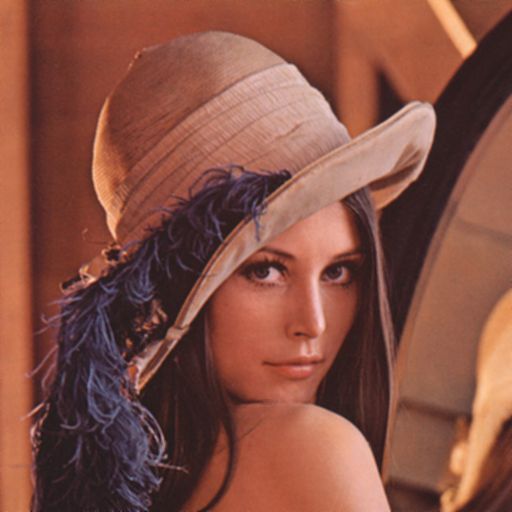
\includegraphics[width=\linewidth]{lenablurc.png}
  \caption{Blur C}
\endminipage\hfill
\minipage{0.2\textwidth}
  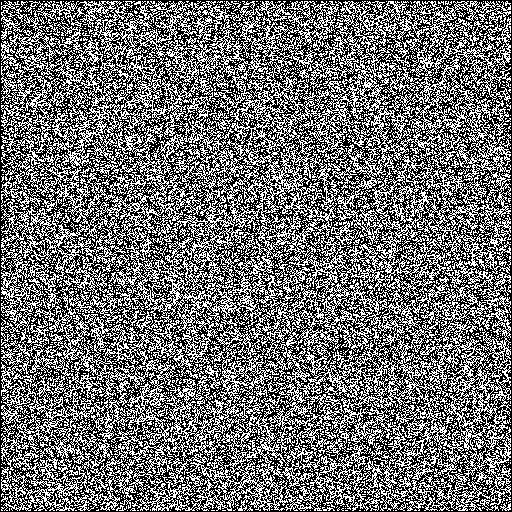
\includegraphics[width=\linewidth]{lenablurdiffR.png}
  \caption{R channel}
\endminipage\hfill
\minipage{0.2\textwidth}
  
\includegraphics[width=\linewidth]{lenablurdiffG.png}
  \caption{G channel}
\endminipage\hfill
\minipage{0.2\textwidth}
  
\includegraphics[width=\linewidth]{lenablurdiffB.png}
  \caption{B channel}
\endminipage\hfill
\minipage{0.2\textwidth}%
  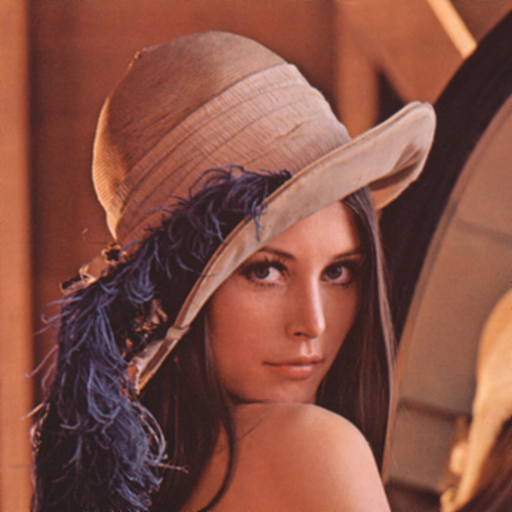
\includegraphics[width=\linewidth]{lenablurasm1.png}
  \caption{Blur ASM}
\endminipage
\end{figure}

Aunque las imágenes parecían exactamente iguales, habían diferencias en algunos píxeles. Estas diferencias se debían al redondeo hacia arriba llevado a cabo por la conversión desde float a entero. Mientras que el código en C redondeaba hacia abajo por defecto, las conversiones en ASM redondeaban hacia arriba por defecto.

Para resolver esto, existe un flag de SSE llamado $MXCSR$. Para mas información, ver la sección 10.2.3.1 del Volumen 1 de la guía de arquitectura Intel. Cada bit de este flag codifica algún comportamiento de las operaciones SSE. El valor por defecto de este flag es $0x1F80$. Para que redondee hacia abajo, utilizando la codificación de los bits del flag, había que poner el bit 12 y 13 en 1. Por lo tanto, simplemente setteamos el flag con la instrucción $ldmxcsr$ en $0x7F80$ y el algoritmo comenzó a andar sin problemas. Tuvimos esta misma problemática en todos los otros filtros más tarde.

\subsection{Experimentación}

Es fácil darse cuenta, ya sea mirando el código o comprendiendo qué es lo que debe hacer el algoritmo de Blur, de que todas las implementaciones del mismo van tener una complejidad temporal de $O(w*h)$, indicando que la cantidad de operaciones que realizará el algoritmo serán de orden cuadrático si tomamos $w = h = n$. Es decir, los gráficos que generemos deberán tener la forma de una parábola a medida que $n$ se vuelva más grande. Lo interesante, y he aquí donde radican las ventajas de hacer el código en Assembler, es que sabemos que las tres implementaciones diferirán en un múltiplo constante de las otras (por la definición de $O$). Intuitivamente, el código de ASM1 debería ir aproximadamente 3 veces más rápido por píxel que el de C, ya que procesa cada canal en paralelo con SIMD, y el código de ASM2 debería ser unas 4 veces más rápido que el de ASM1, ya que no sólo procesa los canales en paralelo, sino que además procesa los píxeles en grupos de a cuatro.

Cabe destacar, de cualquier forma, que nuestra intuición probablemente falle: tanto las optimizaciones que pueda llegar a realizar el compilador de C al código, así como también cuestiones de acceso a memoria en las distintas implementaciones (inclusive las instrucciones utilizadas en cada caso, o el branch predictor), y particularidades respecto del estado actual del sistema en el que se corren los experimentos pueden hacer variar los números obtenidos ampliamente, como veremos más adelante en el caso de HSL.

Haciendo un análisis poco delicado, observemos que la versión de ASM1 tiene 4 saltos condicionales, contra los 5 de ASM2, por lo que en principio, suponiendo que el branch predictor falle, la versión de ASM2 podría terminar siendo más cara. Por otro lado, el hecho de procesar de a 4 píxeles nos dará una ventaja difícil de estimar con respecto al ASM1. En términos del acceso a memoria, ambas versiones hacen uso de la memoria relativamente poco con respecto a los otros algoritmos, entrando solamente con fines de obtener las filas necesarias para procesar los datos, por lo que estimamos que en principio no debería ser el factor más importante, a pesar que todos los accesos que realizamos son desalineados.

Una cosa que nos parece importante resaltar es la manera de la que levantamos los píxeles en la ASM1. Hay muchas formas posibles, por ejemplo, levantar de a 4 siempre, excepto en la última iteración en la que se debe hacer algun malabar para no levantar la parte que causaría un invalid read.
Esta forma uno pensaría que tiene un rendimiento muy superior porque se levantan menos cosas de memoria.
Sin embargo, nuestra primera versión de la implementación levantaba así los pixeles, y tenía el problema del invalid read. Por esa razon, decidimos cambiarnos a la versión actual. La performance no se vió golpeada. Atribuimos esto a que una vez que leimos los datos, estos quedan en la cache, entonces la siguiente lectura va a ser mucho más rápida. Por otro lado, nos ahorramos algunos saltos condicionales que pueden causar algún que otro branch misprediction.


Además, la performance de nuestros algoritmos de Blur no se verá afectada por ninguna otra característica de la imagen que el tamaño: ninguno de los algoritmos actúa según condiciones sobre el contenido de las imágenes. Las tres implementaciones simplemente procesan datos, sin comparar con ninguna otra cosa que no sea el número de columna o de fila. En concreto, esperamos que nuestras implementaciones en Assembler sean ambas más rápidas que la de C, y que entre ellas ASM2 sea más rápida que ASM1 (fundamentalmente por el procesamiento en paralelo de a muchos píxeles).

\begin{figure}[!b]
	\centering
  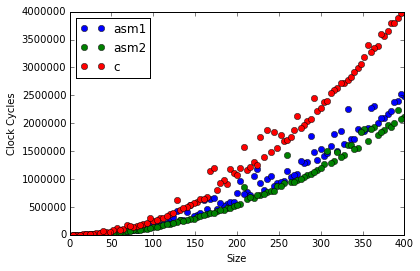
\includegraphics[width=10cm]{blur-imagenes-chicas.png}
  \caption{Performance de C compilado con -o3 y -ffastmath, ASM1 y ASM2. Utilizamos un conjunto de imágenes cuadrádas con tamaños múltiplos de 4 y píxeles tomados de una distribución uniforme, y medimos los resultados de 100 corridas, tomando como estadístico el mínimo de la cantidad de ciclos de reloj en todas las corridas.}
\end{figure}

Observemos que, efectivamente, se cumple lo que esperábamos: los ciclos de reloj crecen de forma cuadrática en relación al tamaño de la imagen. Además, notese que tienen relativamente poco desvío una implementación con respecto a la otra, suponemos que esto quiere decir que tienen comportamientos regulares con respecto al pipeline y sus accesos a memoria (de otra forma, tendríamos más picos en el gráfico). Nos sorprendió mucho que la implementación de ASM1 se asimile tanto a la de ASM2, ya que esperábamos una mayor amplitud entre las curvas; por esto, corrimos un nuevo experimento tomando tamaños de imagen mucho más grandes:

\begin{figure}[!hbt] 
	\centering
  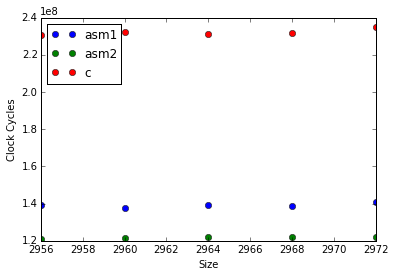
\includegraphics[width=10cm]{blur-imagenes-grandes.png}
  \caption{Performance de C compilado con -o3 y -ffastmath, ASM1 y ASM2. Utilizamos un conjunto de imágenes cuadradas con tamaños múltiplos de 4 y píxeles tomados de una distribución uniforme, y medimos los resultados de 100 corridas, tomando como estadístico el mínimo de la cantidad de ciclos de reloj en todas las corridas.}
\end{figure}

Esta vez, encontramos una brecha mucho más marcada entre las distintas implementaciones, lo que nos asegura que efectivamente el crecimiento de las constantes escondidas en la complejidad temporal está haciendo una diferencia importante a medida que aumenta la escala. Para finalizar, tomamos un ejemplo más de cerca para observar más precisamente las disparidades:

\begin{figure}[!hbt] 
	\centering
  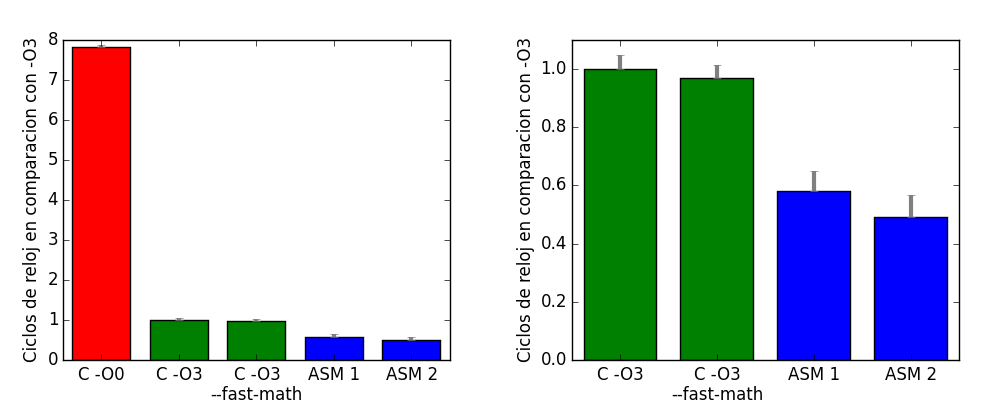
\includegraphics[width=17cm]{blur-all.png}
  \caption{Performance de C compilado con -o0, C compilado con -o3 y -ffastmath, ASM1 y ASM2. Utilizamos una imagen roja de $400 \times 400$, con píxeles tomados de una distribución uniforme, y medimos los resultados de 100 corridas, tomando como estadístico el mínimo de la cantidad de ciclos de reloj en todas las corridas.}
\end{figure}

Como habíamos notado antes, el hecho de estar utilizando imágenes pequeñas no ayuda a que se note la diferencia entre ASM1 y ASM2. Pensamos que uno de los posibles motivos para esto es que los algoritmos que escribimos no están optimizados en tanto a sus accesos a memoria: ambos hacen accesos desalineados. Una posible mejora para el algoritmo de ASM2 sería utilizar los registros AVX para poder obtener más píxeles de memoria, disminuyendo la cantidad de accesos, y permitiéndonos un trabajo mucho más rápido, procesando de a 8 píxeles en simultaneo. Otra posible mejora sería pedir que las direcciones de memoria con las que trabajamos estén alineadas a 16 bits. Esto nos permitiría realizar siempre accesos alineados, lo que debería mejorar la performance de nuestros algoritmos.

